% verso e anverso:
% \documentclass[12pt,openright,twoside,a4paper,english]{abntex2}
% apenas verso: 
\documentclass[12pt,oneside,a4paper,english]{abntex2}


\usepackage{cmap}				% Mapear caracteres especiais no PDF
\usepackage{lmodern}			% Usa a fonte Latin Modern			
\usepackage[T1]{fontenc}		% Selecao de codigos de fonte.
\usepackage[utf8]{inputenc}		% Codificacao do documento (conversão automática dos acentos)
\usepackage{lastpage}			% Usado pela Ficha catalográfica
\usepackage{indentfirst}		% Indenta o primeiro parágrafo de cada seção.
\usepackage{color}				% Controle das cores
\usepackage[table]{xcolor}
\usepackage{graphicx}			% Inclusão de gráficos
\usepackage{pdfpages}
\usepackage[brazilian,hyperpageref]{backref}	 % Paginas com as citações na bibl
\usepackage[alf]{abntex2cite}	% Citações padrão ABNT

\usepackage{listings}
\usepackage{color}
\usepackage{float}

\definecolor{mygreen}{rgb}{0,0.6,0}
\definecolor{mygray}{rgb}{0.5,0.5,0.5}
\definecolor{mymauve}{rgb}{0.58,0,0.82}

\lstdefinelanguage{rock}
{
  morekeywords ={const, typedef, tipo, struct, begin, end, inteiro, function, program, if, then, else, while, do, scan, print, int, float, void, char, bool},
  sensitive = true,
  morecomment = [s]{\%}{\%},
  morestring = [b]",
}

\lstset{ %
  backgroundcolor=\color{white},   % choose the background color; you must add \usepackage{color} or \usepackage{xcolor}
  basicstyle=\footnotesize,        % the size of the fonts that are used for the code
  breakatwhitespace=false,         % sets if automatic breaks should only happen at whitespace
  breaklines=true,                 % sets automatic line breaking
  captionpos=b,                    % sets the caption-position to bottom
  commentstyle=\color{mygreen},    % comment style
  deletekeywords={...},            % if you want to delete keywords from the given language
  escapeinside={\%*}{*)},          % if you want to add LaTeX within your code
  extendedchars=true,              % lets you use non-ASCII characters; for 8-bits encodings only, does not work with UTF-8
  frame=single,                    % adds a frame around the code
  keepspaces=true,                 % keeps spaces in text, useful for keeping indentation of code (possibly needs columns=flexible)
  keywordstyle=\color{blue},       % keyword style
  language=rock,
  numbers=left,                    % where to put the line-numbers; possible values are (none, left, right)
  numbersep=5pt,                   % how far the line-numbers are from the code
  numberstyle=\tiny\color{mygray}, % the style that is used for the line-numbers
  rulecolor=\color{black},         % if not set, the frame-color may be changed on line-breaks within not-black text (e.g. comments (green here))
  showspaces=false,                % show spaces everywhere adding particular underscores; it overrides 'showstringspaces'
  showstringspaces=false,          % underline spaces within strings only
  showtabs=false,                  % show tabs within strings adding particular underscores
  stepnumber=1,                    % the step between two line-numbers. If it's 1, each line will be numbered
  stringstyle=\color{mymauve},     % string literal style
  tabsize=2,                       % sets default tabsize to 2 spaces
  title=\lstname                   % show the filename of files included with \lstinputlisting; also try caption instead of title
}

% Configurações do pacote backref
% Usado sem a opção hyperpageref de backref
\renewcommand{\backrefpagesname}{Citado na(s) página(s):~}
% Texto padrão antes do número das páginas
\renewcommand{\backref}{}
% Define os textos da citação
\renewcommand*{\backrefalt}[4]{
	\ifcase #1 %
		Nenhuma citação no texto.%
	\or
		Citado na página #2.%
	\else
		Citado #1 vezes nas páginas #2.%
	\fi}%

\definecolor{blue}{RGB}{41,5,195} % alterando o aspecto da cor azul

\makeatletter
\hypersetup{
     	%pagebackref=true,
		pdftitle={\@title}, 
		pdfauthor={\@author},
    	pdfsubject={\@title},
		pdfkeywords={Compiladores}, 
		colorlinks=true,       		% false: boxed links; true: colored links
    	linkcolor=blue,          	% color of internal links
    	citecolor=blue,        		% color of links to bibliography
    	filecolor=magenta,      		% color of file links
		urlcolor=blue,
		bookmarksdepth=4
}
\makeatother

\autor{Alan D. Barroso, Kenji Sakata Jr}
\title{Entrega 5 - Tradução dos Comandos}
\orientador[]{Linguagens e Compiladores \\ PCS2056}
\instituicao{%
	Universidade de São Paulo
	\par
	Escola Politécnica}
\local{São Paulo}
\data{2013}

\setlrmarginsandblock{4cm}{4cm}{*}
\setulmarginsandblock{4cm}{4cm}{*}
\checkandfixthelayout

\setlength{\parindent}{1.3cm} % O tamanho do parágrafo
\setlength{\parskip}{0.2cm}  % Controle do espaçamento entre um parágrafo e outro

\SingleSpacing

\makeindex

\begin{document}

\frenchspacing % Retira espaço extra obsoleto entre as frases.

\imprimirfolhaderosto

\clearpage

\textual

\chapter{Analisador Semântico}
  \label{chap:semantico}
    % !TEX encoding = UTF-8 Unicode

\section{Ambiente de Execução}
  \label{chap:ambiente}
    % !TEX encoding = UTF-8 Unicode

\subsection{Elementos da Arquitetura de Von Neumann}
  \label{chap:el_von_neumann}

O compilador da nossa linguagem terá como linguagem de saída um programa escrito especialmente para ser executado dentro de uma maquina virtual intitulada MVN.


O programa MVN é uma abstração da arquitetura de computadores conhecida como arquitetura de Von Neumann. 


Em 1936, o inglês Alan M. Turing propôs um modelo de computação (Máquina de Turing), que compõe-se de:
\begin{itemize}
	\item Uma fita infinita, composta de células, cada qual contendo um símbolo de um alfabeto finito disponível (a fita também implementa a memória externa da máquina).
	\item Um cursor, que pode efetuar leitura ou escrita em uma célula, ou mover-se para a direita ou para a esquerda.
	\item Uma máquina de estados finitos, que controla o cursor.
\end{itemize}


No entanto, a Máquina de Turing apresenta alguns problemas práticos, como:
\begin{itemize}
	\item A Máquina de Turing se apresenta através de um formalismo poderoso, com fita infinita e apenas quatro operações triviais: ler, gravar, avançar e recuar.
	\item Isso faz dela um dispositivo detalhista que oferece apenas uma visão microscópica da solução do problema que pretende resolver, não permitindo ao usuário usar abstrações.
	\item Embora a Máquina de Turing Universal permita uma espécie de programação, o seu código é extenso e a sua velocidade final de execução, muito baixa.
\end{itemize}


A arquitetura de Von Neumann foi em uma alternativa prática viável à Máquina de Turing, disponibilizando operações mais poderosas e ágeis que o modelo de Turing. Assim, ela pode ser considerada como sua evolução natural. Isso pode ser contastado pelas seguintes características:
\begin{itemize}
	\item Memória endereçável, usando acesso aleatório
	\item Programa armazenado na memória, para definir diretamente a função corrente da máquina (ao invés da Máquina de Estados Finitos)
	\item Dados representados na memória (ao invés da fita)
	\item Codificação numérica binária em lugar da unária
	\item Instruções variadas e expressivas para a realização de operações básicas muito freqüentes (ao invés de sub-máquinas específicas)
	\item Maior flexibilidade para o usuário, permitindo operações de entrada e saída, comunicação física com o mundo real e controle dos modos de operação da máquina 
\end{itemize}


Note que sua principal característica é que não há divisão entre dados e o código-fonte do programa em si; ambos são escritos em memória. 


O modelo da arquitetura pode ser melhor compreendido pelo esquema abaixo:

\begin{figure}[H]
	\centering 
	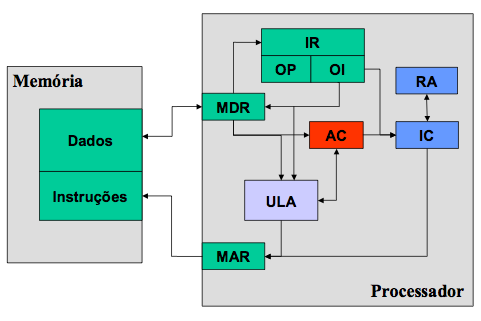
\includegraphics[width=0.8\textwidth]{img/von_neumann.png}  
	\caption{Diagrama da arquitetura de Von Neumann}
	\label{fig:von_neumann}
\end{figure}

A arquitetura de Von Neumann é composta por um processador e uma memória principal. 


Como mostrado anteriormente, na memória principal armazenam-se as intruções do código-fonte e os dados, sendo a divisão mostrada no esquema inexistente (utilizada para fins elucidativos).


Além da ULA (Unidade Lógica Aritmética), a qual é a responsável pelo processamento de operações lógicas e aritméticas, o processador possui um conjunto de elementos físicos de armazenamento de informações e é recorrente dividir esses componentes nos seguintes módulos resgistradores:
\begin{enumerate}
	\item \textbf{MDR -  Registrador de dados da memória}
	

	Serve como ponte para os dados que trafegam entre a memória e os outros elementos da máquina.

	\item \textbf{ MAR - Registrador de endereço de memória}
	

	Indica qual é a origem ou o destino, na memória principal, dos dados contidos no registrador de dados de memória.	

	\item \textbf{IC - Registrador de endereço da próxima instrução }
	

	Indica a cada instante qual será a próxima instrução a ser executada pelo processador.

	\item \textbf{IR -  Registrador de instrução}
	

	Contém a instrução atual a ser executada. É subdividido em dois outros registradores.
	\begin{figure}[H]
		\centering 
		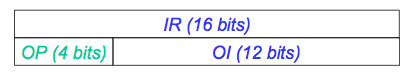
\includegraphics[width=0.8\textwidth]{img/ir.png}  
		\caption{Registrador de Instrução}
		\label{fig:ir}
	\end{figure}


	\begin{enumerate}
		\item \textbf{OP - Registrador de código de operação}


		Parte do registrador de instrução que identifica a instrução que está sendo executada.

		\item \textbf{OI - Registrador de operando de instrução}


		Complementa a instrução indicando o dado ou o endereço sobre o qual ela deve agir.
	\end{enumerate}

	\item \textbf{RA - Registrador de endereço de retorno}
	

	Guarda o endereço da sub-rotina ou função em execução.

	\item \textbf{AC - Acumulador}
	

	Funciona como a área de trabalho para execução de operações lógicas ou aritméticas, acumula o resultado de tais operações.

			 	 	 		
	O conjunto de dados nos registradores contidos em cada instante constitui o estado instantâneo  do processamento. Note que a máquina virtual MVN não realiza diretamente operações lógicas e não há endereçamento indireto nem indexado. Para realizar isso, é preciso realizar algumas manipulações no programa fonte de maneira conveniente.

	
	O funcionamento da máquina funciona em quatro fases:
	\begin{enumerate}
		\item \textbf{Determinação da Próxima Instrução a Executar}

		\item \textbf{Fase de Obtenção da Instrução}


		Obter na memória, no endereço contido no registrador de Endereço da Próxima Instrução, o código da instrução desejada

		\item \textbf{Fase de Decodificação da Instrução}


		Decompor a instrução em duas partes: o código da instrução e o seu operando, depositando essas partes nos registradores de instrução e de operando, respectivamente.


		Selecionar, com base no conteúdo do registrador de instrução, um procedimento de execução dentre os disponíveis no repertório do simulador (passo d). 

		\item \textbf{Fase de Execução da Instrução}


		Executar o procedimento selecionado em (c), usando como operando o conteúdo do registrador de operando, preenchido anteriormente.

		Caso a instrução executada não seja de desvio, incrementar o registrador de endereço da próxima instrução a executar. Caso contrário, o procedimento de execução já terá atualizado convenientemente tal informação.

		\begin{enumerate}
			\item \textbf{Execução da instrução (decodificada em (c))}


			De acordo com o código da instrução a executar (contido no registrador de instrução), executar os procedimentos de simulação correspondentes (detalhados adiante)

			\item \textbf{Acerto do registrador de Endereço da Próxima Instrução para apontar a próxima instrução a ser simulada:}

			Incrementar o registrador de Endereço da Próxima Instrução.
		\end{enumerate}

	\end{enumerate}

\end{enumerate}

\subsection{Instruções da MVN}
  \label{chap:inst_mvn}

As instruções da MVN podem ser resumidas pela seguinte tabela:

\begin{figure}[H]
	\centering 
	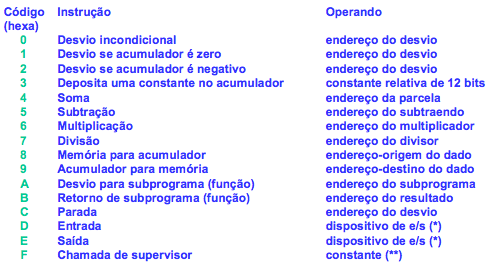
\includegraphics[width=0.9\textwidth]{img/inst_mvn.png}  
	\caption{Instruções da MVN}
	\label{fig:inst_mvn}
\end{figure}

\textbf{Obs.}: Sistema de numeração e aritmética adotada: Binário, em complemento de dois
– representa inteiros e executa operações em 16 bits. O bit mais à esquerda é o bit de sinal (1 = negativo)


A seguir descreveremos o que a máquina realiza ao executar cada tipo de operação: 


\textbf{Registrador de instrução = 0 (desvio incondicional)}


Modifica o conteúdo do registrador de Endereço da Próxima Instrução (IC) armazenando nele o conteúdo do registrador de operando (OI)


IC := OI


\textbf{Registrador de instrução = 1 (desvio se acumulador é zero)}


Se o conteúdo do acumulador (AC) for zero, então modifica o conteúdo do registrador de Endereço da Próxima Instrução (IC), armazenando nele o conteúdo do registrador de operando (OI) 


Se AC = 0 então IC := OI 


Se não IC := IC + 1 


\textbf{Registrador de instrução = 2 (desvio se negativo)}


Se o conteúdo do acumulador (AC) for negativo, isto é, se o bit mais significativo for 1, então modifica o conteúdo do registrador de Endereço da Próxima Instrução  (IC) armazenando nele o conteúdo do registrador de operando (OI)


Se AC < 0 então IC := OI 


Se não IC := IC + 1


\textbf{Registrador de instrução = 3 (constante para acumulador)}


Armazena no acumulador (AC) o número relativo de 12 bits contido no registrador de operando (OI), estendendo seu bit mais significativo (bit de sinal) para completar os 16 bits do acumulador
		

AC := OI 


IC := IC +1 


\textbf{Registrador de instrução = 4 (soma)}


Soma ao conteúdo do acumulador (AC) o conteúdo da posição de memória indicada pelo registrador de operando MEM[OI]. Guarda o resultado no acumulador


AC := AC + MEM[OI] 


IC := IC + 1


\textbf{Registrador de instrução = 5 (subtração)}


Subtrai do conteúdo do acumulador (AC) o conteúdo da posição de memória indicada pelo registrador de operando MEM[OI]. Guarda o resultado no acumulador


AC := AC - MEM[OI]


IC := IC + 1 
		

\textbf{Registrador de instrução = 6 (multiplicação)}


Multiplica o conteúdo do acumulador (AC) pelo conteúdo da posição de memória indicada pelo registrador de operando MEM[OI]. Guarda o resultado no acumulador


AC := AC * MEM[OI] 


IC := IC + 1


\textbf{Registrador de instrução = 7 (divisão inteira)}


Dividir o conteúdo do acumulador (AC) pelo conteúdo da posição de memória indicada pelo registrador de operando MEM[OI]. Guarda a parte inteira do resultado no acumulador


AC := int (AC / MEM[OI])


IC := IC + 1 
			

\textbf{Registrador de instrução = 8 (memória para acumulador)}


Armazena no acumulador (AC) o conteúdo da posição de memória endereçada pelo registrador de operando (OI) 


AC := MEM[OI]		


IC := IC + 1
			

\textbf{Registrador de instrução = 9 (acumulador para memória)}


Guarda o conteúdo do acumulador (AC) na posição de memória endereçada pelo registrador de operando (OI) 


MEM[OI] := AC		


IC := IC + 1 
			

\textbf{Registrador de instrução = A (desvio para subprograma)}


Armazena o conteúdo do registrador de Endereço da Próxima instrução (IC), incrementado de uma unidade, no registrador de endereço de retorno (RA).


Armazena no registrador de Endereço da Próxima instrução (IC) o conteúdo do registrador de operando (OI).


RA := IC + 1


IC := OI


\textbf{Registrador de instrução = B (retorno de subprograma)}


Armazena no registrador de Endereço da Próxima instrução (IC) o conteúdo do registrador de endereço de retorno (RA), e no acumulador (AC) o conteúdo da posição de memória apontada pelo registrador de operando (OI) 


AC := MEM[OI]			


IC := RA 	 	 	 		
			

\textbf{Registrador de instrução = A (desvio para subprograma)}				 					


Armazena o conteúdo do registrador de Endereço da Próxima instrução (IC), incrementado de uma unidade, na posição de memória endereçada pelo registrador de operando (OI), que corresponde ao endereço do subprograma.				


Armazena no registrador de Endereço da Próxima instrução (IC) o conteúdo do registrador de operando (OI), incrementado de uma unidade.


MEM[OI] := IC + 1


IC := OI + 1 


\textbf{Registrador de instrução = B (retorno de subprograma)}
			

Recupera no registrador de endereço de retorno (RA) o conteúdo da posição de memória apontada pelo registrador de operando (OI), que vem a ser o endereço de retorno.


Armazena no registrador de Endereço da Próxima instrução (IC) o conteúdo do registrador de endereço de retorno (RA).


RA := MEM[OI]


IC := RA 

		 	 	 		
			
\textbf{Registrador de instrução = C (stop)}


Modifica o conteúdo do registrador de Endereço da Próxima instrução (IC) armazenando nele o conteúdo do registrador de operando (OI) e para o processamento


IC := OI 


Para

\begin{figure}[H]
	\centering 
	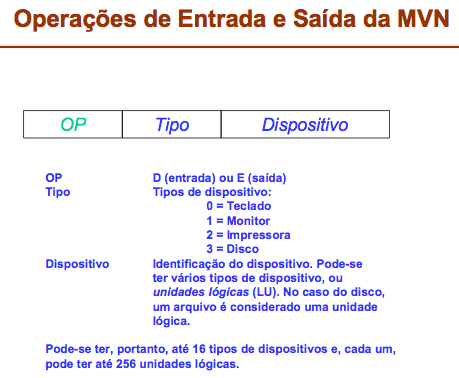
\includegraphics[width=0.8\textwidth]{img/input_output.png}  
	\caption{Instruções de entrada e saída}
	\label{fig:input_output}
\end{figure}

\textbf{Registrador de instrução = D (input)}
 					

Aciona o dispositivo padrão de entrada e aguardar que o usuário forneça o próximo dado a ser lido.


Transfere o dado para o acumulador 


Aguarda


AC := dado de entrada 


IC := IC + 1 
		

\textbf{Registrador de instrução = E (output)}


Transfere o conteúdo do acumulador (AC) para o dispositivo padrão de saída.
Aciona o dispositivo padrão de saída e aguardar que este termine de executar a operação de saída 


dado de saída := AC 


aguarda


IC := IC + 1


\textbf{Registrador de instrução = F (supervisor call)}


Não implementado: por enquanto esta instrução não faz nada.


IC := IC + 1

\subsection{Módulos Extras: Montador, Ligador e Relocador}
  \label{chap:extras}

O compilador traduz o código-fonte da linguagem de alto nível em código-objeto. Tal código não é escrito em linguagem de máquina, executável pela máquina de Von Neumann. 


Na realidade, ele é escrito em linguagem de montagem (simbólica). Essa linguagem é bastante próxima da linguagem de máquina, mas é mais compreensível por um ser humano, por ser mais legível. Isso deve-se ao fato de que as instruções não são descritas por números hexadecimais, mas por mnemônicos os quais representam de maneira mais intuitiva o significado de cada instrução.


Os mnemônicos para a MVN estão resumidos na seguinte tabela:

\begin{figure}[H]
	\centering 
	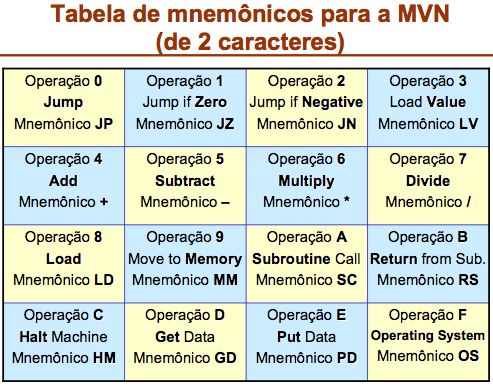
\includegraphics[width=0.8\textwidth]{img/mnemonicos.png}  
	\caption{Mnemônicos}
	\label{fig:mnemonicos}
\end{figure}

O elemento responsável por traduzir o código-objeto em linguagem de máquina é o Montador (Assembler). Em seguida, o resultado (que não está completamente resolvido e ainda não tem seu endereço definido) é repassado para o Ligador (Linker), o qual é o responsável por resolver a modularização dos programas (uso de bibliotecas). Por exemplo, quando do uso de funções ou subrotinas de programas externos dentro da execução de um programa principal.


Finalmente, o resultado do Ligador é repassado ao Relocador, possibilitando que os programas a serem executados pela máquina de Von Neumann possam ser devidamente relocados convenientemente pelo sistema operacional na memória principal. Isso evita o problema de programas absolutos que devem ser executados estritamente nas posições de memória em que foram criados, consistindo em um risco de uso potencialmente indevido da memória.


Esse módulos extras são entidades à parte da arquitetura de Von Neumann, mas a implementação da MVN que estamos utilizando no projeto, já os possui devidamente integrados, de forma que é possível realizar a execução de um código-objeto fornecido pelo compilador que está escrito na linguagem simbólica de montagem.


\subsection{Pseudo-instruções da Linguagem de Montagem}
  \label{chap:pseudo_instrucoes}


A linguagem simbólica do código-objeto não possui somente os mnemônicos das instruções da MVN, pois é necessário lidar com os endereços dentro de um programa (rótulos, operandos, sub-rotinas), com a reserva de espaço para tabelas, com valores constantes. 


Assim, há comandos chamados de pseudo-instruções da linguagem de montagem. Eles são chamados dessa forma porque não representam efetivamente as instruções da máquina de Von Neumann, mas são necessários para resolver os problemas evocados anteriormente.


Na linguagem de montagem, as pseudo-instruções também são representadas por mnemônicos. São eles:

\begin{itemize}
	\item \textbf{@} : Origem Absoluta. Recebe um operando numérico, define o endereço da instrução seguinte.
	\item \textbf{K} : Constante, o operando numérico tem o valor da constante (em hexadecimal). Define uma área preenchida por uma CONSTANTE de 2 bytes
	\item \textbf{\$} : Reserva de área de dados, o operando numérico define o tamanho da área a ser reservada. Define um BLOCO DE MEMÓRIA com número especificado de words.
	\item \textbf{\#} : Final físico do texto fonte.
	\item \textbf{\&} : Origem relocável
	\item \textbf{>} : Endereço simbólico de entrada (entry point). Define um endereço simbólico local como entry-point do programa.
	\item \textbf{<} : Endereço simbólico externo (external). Define um endereço simbólico que referencia um entry-point externo.
\end{itemize}

 
 Assim, com esses elementos, é possível obter-se o código de máquina a partir do código-objeto. A seguir, temos um exemplo de um código escrito em linguagem de montagem e sua respectiva tradução pelos módulos Montador, Logador e Relocador:

\begin{figure}[H]
	\centering 
	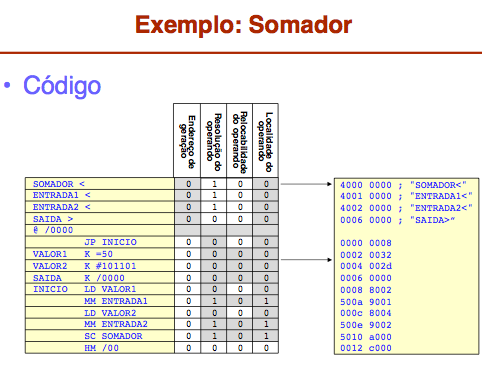
\includegraphics[width=0.8\textwidth]{img/somador.png}  
	\caption{Exemplo: somador}
	\label{fig:somador}
\end{figure}

\subsection{Descrição Geral do Ambiente de Execução}
  \label{chap:descricao_ambiente}

\subsubsection{Organização da memória}
  \label{chap:org_memoria}

O ambiente de execução da MVN fornece aos programadores um total de 4Kb de memória para ser usado tanto para o código quanto para as variáveis do programa. O montador aloca a memória com base nos endereços relativos especificados no código do programa. Desses 4Kb, a parte inicial da memória é reservada para guardar as instruções que serão executadas pelo programa. A parte final da memória deve ser usada especialmente para o uso do registro de ativação.


Em outras palavras, reserva-se uma parte do código para a área de dados, onde se encontram as variáveis, uma parte para o resto do programa, que inclui a função principal e as subrotinas e uma parte dedicada a pilhas de variáveis e endereços que viabilizam a chamada de subrotinas.

\subsubsection{Funções de Input e Output}
  \label{chap:in_out}

As funções de Input e Output serão implementadas na MVN. Serão fornecidas três funções de input e duas de output:

\begin{itemize}
	\item GET\_CHAR: Devolve um caracter lido na entrada do teclado

	\item GET\_STRING: Pega um conjunto de caracteres, sem contar os espaços, tabs e saltos de linha
	
	\item GET\_NUMBER: Captura um número no formato ASCII e devolve sob a forma de hexadecimal
	
	\item PRINT\_STRING: Imprime uma cadeia de caracteres
	
	\item PRINT\_NUMBER: Transforma um número hexadecimal em caracteres ASCII
\end{itemize}

\subsubsection{Registro de ativação}
  \label{chap:in_out}

As subrotinas são executadas com as seguintes instruções da MVN:

\begin{itemize}
	\item Desvio para subprograma (função) - código SC (A): armazena o endereço de instrução seguinte (atual + 1)  na posição de memória apontada pelo operando. Em seguida, desvia a execução para o endereço indicado pelo operando e acrescido de uma unidade.
	\item Retorno de subprograma (função) - código RS (B): desvia a execução para o endereço indicado pelo valor guardado na posição de memória do operando.
\end{itemize}

Para garantir a operação de chamar várias subrotinas aninhadas (ex.: recursões), é necessário empilhar as variáveis do programa, isto é, o estado da execução do programa e também a quantidade de variáveis da rotina em execução (valor guardado na área auxiliar). Para tanto, utilizamos a estrutura chamada de Registro de Ativação.


O registro de ativação nesse ambiente de execução será feito sob a forma de uma pilha, onde a cada chamada de função todos os dados do referentes a função, bem como o endereço de retorno, devem ser empilhados para serem usados. Os dados a serem empilhados no registro de ativação são:

\begin{itemize}
	\item Endereço de retorno
	\item Endereço do próximo endereço da pilha
	\item Parâmetros da função
	\item Variáveis locais das função
\end{itemize}

O endereço de retorno fica localizado no primeiro endereço do bloco empilhado no registro de ativação. O segundo endereço é referente ao endereço do primeiro endereço do próximo bloco do registro de ativação. Esse endereço é usado para mudar o valor ponteiro do registro de ativação, para que a função que chamou a outra possa voltar a enxergar suas variáveis. Do terceiro endereço em diante estão localizados os parâmetros da função. Após o final dos parâmetros, estão localizadas as variáveis locais necessárias para guardar executar as operações durante a execução da função.


Os endereços das variáveis locais e dos parâmetros podem ser calculados usando o ponteiro do registro de ativação, somando dois mais os tamanhos das variáveis existentes anteriormente.


A figura a seguir ilustra a organização da pilha de ativação.

\begin{figure}[H]
	\centering 
	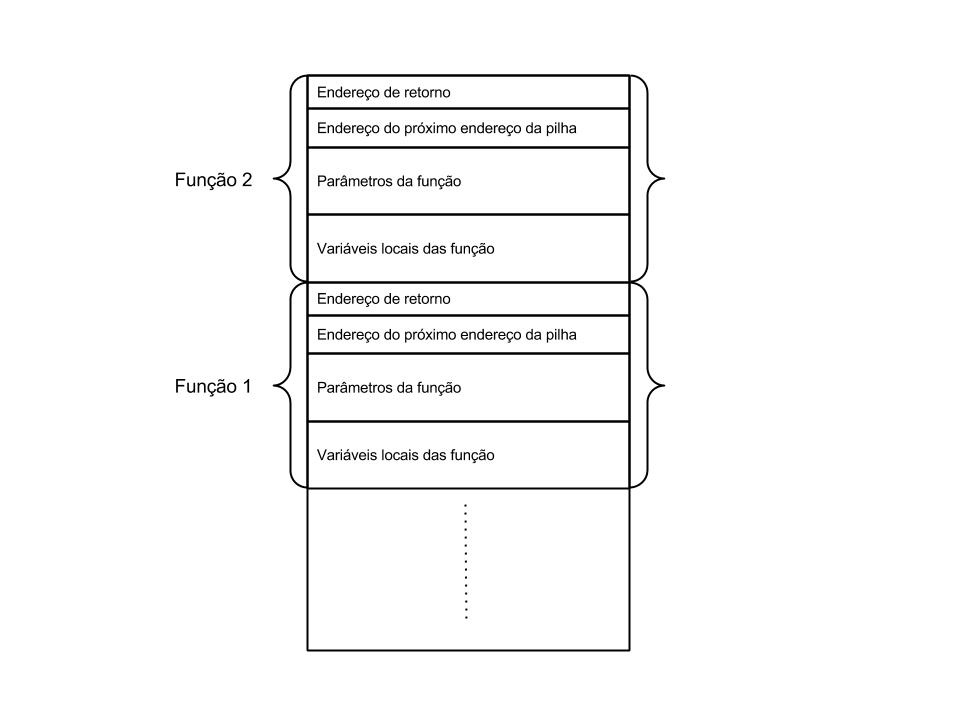
\includegraphics[width=0.9\textwidth]{img/registro_ativacao.png}  
	\caption{Registro de Ativação}
	\label{fig:registro_ativacao}
\end{figure}

O uso do registro de ativação permite entre outras coisas a chamada recursiva de funções, uma vez isso não é possível de forma nativa no ambiente da MVN. Com registro de ativação, realizar uma recursão significa empilhar um novo bloco à pilha e relançar a execução da função.


Para implementar o registro de ativação, tivemos de desenvolver uma bibliteca nativa ao compilador em linguagem de montagem (Assembly).


Basicamente, a biblioteca implementa uma pilha, onde os nós são as informações guardadas no registro de ativação.
Uma dificuldade que encontramos foi a de copiar os dados de uma função para a pilha, pois devemos transmitir o conteúdo de um ponteiro para outro. 


Para facilitar o processo de montagem, ligação e relocação utilizamos um script de nosso colega Gustavo Pacianotto Gouveia, o qual realiza automaticamente a conversão de nosso código Assembly em linguagem MVN (de máquina).

\section{Traduções de comandos semânticos para linguagem MVN}
  \label{chap:traducao}
    % !TEX encoding = UTF-8 Unicode
\definecolor{light-gray}{gray}{0.95}
\definecolor{non-photoblue}{rgb}{0.64, 0.87, 0.93}

\subsection{Tradução dos comandos imperativos}

\textbf{Nota}: <expressao> trata-se de um abuso de linguagem, pois na realidade precisamos guardar o valor calculado - que está no acumulador - em uma variável temporária e depois utilizá-la sempre qquando utilizamos <expressao> diretamente.

\begin{table}[H]
	\rowcolors{1}{light-gray}{white}

	\begin{tabular}{ | p{3cm} | p{5cm} | p{5cm}|}
	\rowcolor{non-photoblue}
	\textbf{Comando} & \textbf{Linguagem} & \textbf{MVN Simbólica} \\
	
	\hline
	
	Declaração de variável escalar simples & int x; & x K /0000 \\

	Declaração de variável vetorial simples & int x[n]; & x \$ =n \\

	Declaração de estrutura simples & struct s begin\newline int p1;\newline int p2;\newline int p3[n];\newline end struct\newline\newline s x; & x K /0000\newline K /0000\newline \$ =n \\

	\hline
	\end{tabular}
	\caption{Tradução dos comandos principais para a MVN: Parte I}
\end{table}


\begin{table}[H]
	\rowcolors{1}{light-gray}{white}

	\begin{tabular}{ | p{3cm} | p{5cm} | p{5cm}|}
	\rowcolor{non-photoblue}
	\textbf{Comando} & \textbf{Linguagem} & \textbf{MVN Simbólica} \\
	
	\hline

	Atribuição de variável escalar ou de estrutura & x = <expressao>; &  LV x\newline + n ; n > 0 para struct\newline\ MM END\_ALVO\newline\newline <expressao>\newline\newline LD <expressao>\newline MM VALOR\newline\newline SC GRAVA \\

	Atribuição de variável vetorial & x[<expressao>] = <expressao>; & <expressao>\newline\newline LV x\newline + <expressao>\newline MM END\_ALVO\newline\newline <expressao>\newline\newline LD <expressao>\newline MM VALOR\newline\newline SC GRAVA \\

	Acesso à variável vetorial & x[<expressao>] & <expressao>\newline\newline LV x \newline + <expressao>\newline MM END\_ORIGEM\newline SC ACESSA \\

	\hline
	\end{tabular}
	\caption{Tradução dos comandos principais para a MVN: Parte II}
\end{table}

\begin{table}
	\rowcolors{1}{light-gray}{white}

	\begin{tabular}{ | p{3cm} | p{5cm} | p{5cm}|}
	\rowcolor{non-photoblue}
	\textbf{Comando} & \textbf{Linguagem} & \textbf{MVN Simbólica} \\
	
	\hline

	Declaração de função & function int func(int p1, char p2) begin\newline\newline<comandos>\newline\newline end function & func\_end\_retorno K /0000\newline K /0000\newline func\_p1 K /0000\newline func\_p2 K /0000\newline\newline TMP1 K /0000\newline TMP2 K /0000\newline...\newline func JP /000\newline <comandos>\newline RS func \\

	Chamada de função & func(<expressao>, <expressao>) & LD parent\newline MM parent\_end\_retorno\newline\newline LV parent\_end\_retorno\newline MM END\_INICIAL\newline\newline LV parent\_tamanho\newline MM TAMANHO\newline\newline SC EMPILHA\newline\newline <expressao>\newline LD <expressao>\newline MM func\_p1\newline\newline <expressao>\newline LD <expressao>\newline MM func\_p2\newline\newline SC func \newline\newline MM TMP\_RETURN\newline\newline LD TOPO \newline MM END\_BLOCO\_ORIGEM\newline\newline LD parent\_end\_retorno\newline MM END\_BLOCO\_ALVO\newline\newline LV parent\_tamanho\newline MM TAMANHO\_BLOCO\newline  SC COPIA\_BLOCO\newline\newline LD TMP\_RETURN \\

	\hline
	\end{tabular}
	\caption{Tradução dos comandos principais para a MVN: Parte III}
\end{table}

\begin{table}[H]
	\rowcolors{1}{light-gray}{white}

	\begin{tabular}{ | p{3cm} | p{5cm} | p{5cm}|}
	\rowcolor{non-photoblue}
	\textbf{Comando} & \textbf{Linguagem} & \textbf{MVN Simbólica} \\
	
	\hline

	Leitura (entrada) & scan x, y, z; & LV x\newline MM END\_ALVO\newline\newline SC SCAN\_INT\newline\newline LV y\newline MM END\_ALVO\newline\newline SC SCAN\_INT\newline\newline LV z\newline MM END\_ALVO\newline\newline SC SCAN\_CHAR \\

	Impressão (saída) & print x, y, z; & LV x\newline MM END\_ORIGEM\newline\newline SC ACESSA\newline MM VAR\newline\newline SC PRINT\_INT\newline\newline LV y\newline MM END\_ORIGEM\newline\newline SC ACESSA\newline MM VAR\newline\newline SC PRINT\_INT\newline\newline LV z\newline MM END\_ORIGEM\newline\newline SC ACESSA\newline MM VAR\newline\newline SC PRINT\_CHAR \\

	\hline
	\end{tabular}
	\caption{Tradução dos comandos principais para a MVN: Parte IV}
\end{table}

\subsection{Tradução de estruturas de controle de fluxo}

\begin{table}[H]
	\rowcolors{1}{light-gray}{white}

	\begin{tabular}{ | p{3cm} | p{5cm} | p{5cm}|}
	\rowcolor{non-photoblue}
	\textbf{Comando} & \textbf{Linguagem} & \textbf{MVN Simbólica} \\
	
	\hline

	If-then & if (<expressao>) then \newline <comandos> \newline end if & TMP K /0001 \newline\newline <expressao>\newline LD <expressao>\newline MM TMP\newline\newline LD TMP\newline JZ ENDIF\newline\newline<comandos>\newline\newline ENDIF \\

	If-then-else & if (<expressao>) then \newline <comandos> \newline else \newline <comandos> \newline end if & TMP K /0001\newline\newline <expressao>\newline LD <expressao>\newline MM TMP\newline LD TMP\newline\newline JZ ELSE\newline<comandos>\newline JP ENDIF\newline\newline ELSE \newline<comandos>\newline ENDIF \\

	While & while (<expressao>) do\newline <comandos>\newline end while & TMP K /0001\newline\newline WHILE\newline\newline<expressao>\newline LD <expressao>\newline MM TMP\newline LD TMP\newline\newline JZ ENDWHILE\newline<comandos>\newline JP WHILE\newline\newline ENDWHILE \\

	\hline
	\end{tabular}
	\caption{Tradução dos comandos principais para a MVN: Parte V}
\end{table}

\subsection{Funções auxiliares}

\subsubsection{Biblioteca auxiliar}

Criamos uma biblioteca auxiliar que permite gerar o código MVN das tabelas anteriores. Ela é carregada em todos os programas compilados pelo compilador que estamos desenvolvendo.


Todas as variáveis auxiliares às quais tivemos de atribuir um valor como VALOR, TAMANHO, END\_ALVO etc. são parâmetros das funções auxiliares.


As principais funções existentes na biblioteca referem-se à implementação de uma pilha (no nosso caso, uma abstração do registro de ativação). Assim, além das tradicionais EMPILHA e DESEMPILHA, temos algumas funções auxiliares que ajudam a implementá-las:

\begin{itemize}
	\item \textbf{COPIA\_BLOCO}: permite copiar o conteúdo de um bloco de código para outro. A cópia se dá de maneira conveniente para o registro de ativação, quer dizer, respeitando a estrutura convencionada.
	\item \textbf{ACESSA}: Coloca no acumulador o valor localizado no ponteiro do endereco de origem.
	\item \textbf{GRAVA}:  Grava no enedereço alvo o valor do parâmetro VALOR.
	\item \textbf{SCAN\_*}: Realiza a leitura do dispotivo de entrada.
	\item \textbf{PRINT\_*}: Imprime sobre o dispositivo de entreda.
\end{itemize}

\textbf{Nota}: Grande parte das manipulações da biblioteca auxiliar usam a noção de ponteiros. Para maiores informações, consultar o código enviado em anexo, o qual encontra-se comentado.

\subsubsection{Cálculo de <expressao>}

Para a geração de código em linguagem MVN, será necessário uma pilha, uma lista,  um contador para variáveis temporárias e um para endereços de desvio para auxílio (label). 


Note que uma expressão pode ser tanto aritmética quanto booleana em nossa linguagem e a ordem de precedência dos operadores é: operações unárias (! ou -), multiplicação/divisão, adição/subtração, comparações lógicas (>, <, >=, <=, ==, !=), operação lógica E, operação lógica OU. 

\begin{enumerate}
	\item Empilha os átomos assim que são lidos para o analisador sintático até encontrar um “)”. 
	
	\item Quando encontrar o “)”, desempilha e coloque na lista auxiliar até encontrar o “(“. Se não houver “)”, vá para o passo 6.

	\item Resolve-se os operadores unários "!" e "-".

	\begin{table}[H]
			\rowcolors{1}{light-gray}{white}

			\begin{tabular}{| p{7cm} | p{8cm}|}
			\rowcolor{non-photoblue}
			\textbf{Linguagem} & \textbf{MVN Simbólica} \\
			
			\hline

			! NUM/ID anterior & LV =NUM ; ou LD ID anterior\newline JZ JUMP\_EXPBOOL<contador>\newline LV =0\newline MM temp<contador de variável temporária>\newline JP FIM\_EXPBOOL<contador>\newline JUMP\_EXPBOOL<contador> LV =1\newline MM temp<contador de variável temporária>\newline FIM\_EXPBOOL<contador> \\

			- NUM/ID anterior & LV =NUM ; ou LD ID anterior\newline MM temp<contador de variável temporária>\newline LV =0\newline - temp<contador de variável temporária>\newline MM temp<contador de variável temporária> \\

			\hline
			\end{tabular}
			\caption{Tradução dos comandos principais para a MVN: multiplicação e divisão}
		\end{table}

	Após a geração do código, deve-se substituir na lista o átomo pela variável temporária criada.

	\item Resolve-se os operadores “*” e “/” percorrendo a lista procurando-os.

		\begin{table}[H]
			\rowcolors{1}{light-gray}{white}

			\begin{tabular}{| p{7cm} | p{8cm}|}
			\rowcolor{non-photoblue}
			\textbf{Linguagem} & \textbf{MVN Simbólica} \\
			
			\hline

			NUM/ID posterior *\_/ NUM/ID anterior & LV  =NUM ; ou LD ID posterior\newline\newline *\_/  <NUM/ID anterior>\newline\newline MM temp<contador de variável temporária> \\

			\hline
			\end{tabular}
			\caption{Tradução dos comandos principais para a MVN: multiplicação e divisão}
		\end{table}


		Após a geração do código, deve-se substituir na lista os três átomos pela variável temporária criada.

	\item Resolve-se os operadores “+” e “-” da mesma forma que no passo 4.

	\begin{table}[H]
			\rowcolors{1}{light-gray}{white}

			\begin{tabular}{| p{7cm} | p{8cm}|}
			\rowcolor{non-photoblue}
			\textbf{Linguagem} & \textbf{MVN Simbólica} \\
			
			\hline

			NUM/ID posterior +\_- NUM/ID anterior & LV  =NUM ; ou LD ID posterior\newline\newline +\_-  <NUM/ID anterior>\newline\newline MM temp<contador de variável temporária> \\

			\hline
			\end{tabular}
			\caption{Tradução dos comandos principais para a MVN: adição e subtração}
	\end{table}


	Após a geração do código, deve-se substituir na lista os três átomos pela variável temporária criada.

	\item Resolve-se os operadores de comparação lógica da mesma forma que no passo 4.

	\begin{table}[H]
			\rowcolors{1}{light-gray}{white}

			\begin{tabular}{| p{7cm} | p{8cm}|}
			\rowcolor{non-photoblue}
			\textbf{Linguagem} & \textbf{MVN Simbólica} \\
			
			\hline

			NUM/ID posterior > NUM/ID anterior & LV =NUM ; ou LD ID posterior\newline - <NUM ou ID anterior>\newline JN JUMP\_EXPBOOL<contador>\newline LV =1\newline MM temp<contador de variável temporária>\newline JP FIM\_EXPBOOL<contador>\newline JUMP\_EXPBOOL<contador> LV =0\newline MM temp<contador de variável temporária>\newline FIM\_EXPBOOL<contador>\newline \\

			NUM/ID posterior < NUM/ID anterior & LV =NUM ; ou LD ID posterior\newline - <NUM ou ID anterior>\newline JN JUMP\_EXPBOOL<contador>\newline LV =0\newline MM temp<contador de variável temporária>\newline JP FIM\_EXPBOOL<contador>\newline JUMP\_EXPBOOL<contador> LV =1\newline MM temp<contador de variável temporária>\newline FIM\_EXPBOOL<contador>\newline \\
			\hline
			\end{tabular}
			\caption{Tradução dos comandos principais para a MVN: comparação lógica}
	\end{table}

	\begin{table}[H]
			\rowcolors{1}{light-gray}{white}

			\begin{tabular}{| p{7cm} | p{8cm}|}
			\rowcolor{non-photoblue}
			\textbf{Linguagem} & \textbf{MVN Simbólica} \\
			
			\hline

			NUM/ID posterior >= NUM/ID anterior & LV =NUM ; ou LD ID posterior\newline - <NUM ou ID anterior>\newline JN JUMP\_EXPBOOL<contador>\newline JZ JUMP\_EXPBOOL<contador>\newline LV =1\newline MM temp<contador de variável temporária>\newline JP FIM\_EXPBOOL<contador>\newline JUMP\_EXPBOOL<contador> LV =0\newline MM temp<contador de variável temporária>\newline FIM\_EXPBOOL<contador>\newline \\

			NUM/ID posterior <= NUM/ID anterior & LV =NUM ; ou LD ID posterior\newline - <NUM ou ID anterior>\newline JN JUMP\_EXPBOOL<contador>\newline JZ JUMP\_EXPBOOL<contador>\newline LV =0\newline MM temp<contador de variável temporária>\newline JP FIM\_EXPBOOL<contador>\newline JUMP\_EXPBOOL<contador> LV =1\newline MM temp<contador de variável temporária>\newline FIM\_EXPBOOL<contador>\newline \\
			\hline
			\end{tabular}
			\caption{Tradução dos comandos principais para a MVN: comparação lógica II}
	\end{table}

	\begin{table}[H]
			\rowcolors{1}{light-gray}{white}

			\begin{tabular}{| p{7cm} | p{8cm}|}
			\rowcolor{non-photoblue}
			\textbf{Linguagem} & \textbf{MVN Simbólica} \\
			
			\hline

			NUM/ID posterior == NUM/ID anterior & LV =NUM ; ou LD ID posterior\newline - <NUM ou ID anterior>\newline JZ JUMP\_EXPBOOL<contador>\newline LV =0\newline MM temp<contador de variável temporária>\newline JP FIM\_EXPBOOL<contador>\newline JUMP\_EXPBOOL<contador> LV =1\newline MM temp<contador de variável temporária>\newline FIM\_EXPBOOL<contador>\newline \\

			NUM/ID posterior != NUM/ID anterior & LV =NUM ; ou LD ID posterior\newline - <NUM ou ID anterior>\newline JZ JUMP\_EXPBOOL<contador>\newline LV =1\newline MM temp<contador de variável temporária>\newline JP FIM\_EXPBOOL<contador>\newline JUMP\_EXPBOOL<contador> LV =0\newline MM temp<contador de variável temporária>\newline FIM\_EXPBOOL<contador>\newline \\

			\hline
			\end{tabular}
			\caption{Tradução dos comandos principais para a MVN: comparação lógica III}
	\end{table}

	Após a geração do código, deve-se substituir na lista os três átomos pela variável temporária criada.

	\item Resolve-se a operação lógica E.

	\begin{table}[H]
			\rowcolors{1}{light-gray}{white}

			\begin{tabular}{| p{7cm} | p{8cm}|}
			\rowcolor{non-photoblue}
			\textbf{Linguagem} & \textbf{MVN Simbólica} \\
			
			\hline

			NUM/ID posterior and NUM/ID anterior & LV =NUM ; ou LD ID posterior\newline * NUM ; ou ID anterior\newline MM temp<contador de variável temporária> \\

			\hline
			\end{tabular}
			\caption{Tradução dos comandos principais para a MVN: operação lógica E}
	\end{table}

	Após a geração do código, deve-se substituir na lista os três átomos pela variável temporária criada.

	\item Resolve-se a operação lógica OU.

	\begin{table}[H]
			\rowcolors{1}{light-gray}{white}

			\begin{tabular}{| p{7cm} | p{8cm}|}
			\rowcolor{non-photoblue}
			\textbf{Linguagem} & \textbf{MVN Simbólica} \\
			
			\hline

			NUM/ID posterior or NUM/ID anterior & LV =NUM ; ou LD ID posterior\newline + NUM ; ou ID anterior\newline JZ JUMP\_EXPBOOL<contador>\newline LV =1\newline MM temp<contador de variável temporária>\newline JP FIM\_EXPBOOL<contador>\newline JUMP\_EXPBOOL<contador> LV =0\newline MM temp<contador de variável temporária>\newline FIM\_EXPBOOL<contador> \\

			\hline
			\end{tabular}
			\caption{Tradução dos comandos principais para a MVN: operação lógica OU}
	\end{table}

	Após a geração do código, deve-se substituir na lista os três átomos pela variável temporária criada.

	\item Quando a lista contiver apenas um item, insira-o na pilha e volte para o passo 1, cujo intuito é o de eliminar mais parênteses.

	\item Nesse passo, a pilha encontra-se com toda a expressão sem parênteses. Com isso, pode-se jogar todo o conteúdo da pilha na lista e resolvê-la com os passos 3 a 8.

	\item Após resolver todos os operadores, a lista estará apenas com um átomo, sendo o resultado da expressão e o código já foi gerado.
	
	LV =NUM ; ou LD ID

\end{enumerate}

    
\end{document}
